%-*-coding: utf-8-*-
\FloatBarrier
\chapter{Описание используемого подхода}

\FloatBarrier
\section{Основная идея}

Идея заключается в составлении булевой формулы для набора входных деревьев и гибридизационного числа $h$, которая выполнима тогда и только тогда, когда существует гибридизационная сеть $N_h$ с гибридизационным числом $h$, содержащая в себе все входные деревья.
Тогда, определив возможные границы гибридизационного числа, можно составить формулы для всех возможных гибридизационных чисел, после чего ответом на задачу будет та из выполнимых формул, соответствующая наименьшему гибридизационному числу.
После этого по формуле восстанавливается структура гибридизационной сети.

\FloatBarrier
\section{Препроцессинг}

Перед тем как приступать к непосредственному кодированию булевой формулы, применяются несколько эвристик, позволяющих разбить задачу на подзадачи, и следовательно уменьшить её сложность.
Для разбиения применяются следующие правила~\cite{bonet2009efficiently}:

\begin{enumerate}
	\item \textbf{Сокращение поддерева.} Если существует поддерево, содержащееся в каждом из исходных деревьев, значит в этой части эволюционной истории не наблюдалось ретикуляций, и для её отображения достаточно древовидной структуры.
	Поэтому во всех исходных деревьях следует заменить это поддерево на лист с новой меткой.
	После решения задачи, в готовой сети, следует заменить этот лист на исходное поддерево.
	\item \textbf{Сокращение кластера.} Если существует кластер $A$, содержащийся в каждом из исходных деревьев, его также следует заменить на лист с новой меткой, а задачу построения минимальной гибридизационной сети решать для этого кластера отдельно.
	После решения задачи, следует заменить этот лист в готовой сети на сеть, являющуюся решением задачи для кластера $A$.
\end{enumerate}

Предложенный далее алгоритм предполагает, что у всех входных деревьев общий корень, но это предположение не выполняется для построенных подзадач.
Поэтому следует добавить фиктивный корень ко всем деревьям в каждой из подзадач.
Чтобы сохранить структуру деревьев корень добавляется вместе с новым фиктивным листом.
Этот процесс проиллюстрирован на Рис.~\ref{dummy-example}.
После решения задачи, фиктивный корень и фиктивный лист следует удалить.

\begin{figure}[t]
  \begin{minipage}[b]{0.49\linewidth}
    \centering{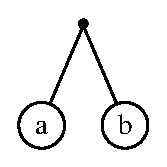
\includegraphics[width=2.6cm]{img/inp_dummy.eps}}
%    \centering{\\ (а) Простое дерево.}
  \end{minipage}
  \hfill
  \begin{minipage}[b]{0.49\linewidth}
  	\centering{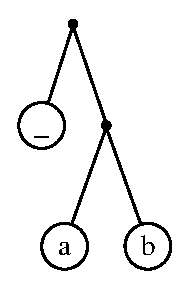
\includegraphics[width=3cm]{img/ans_dummy.eps}}
%    \centering{\\ (б) Дерево с фиктивным корнем и листом.}
  \end{minipage}
  \caption{Добавление фиктивного корня к дереву.}
  \label{dummy-example}
\end{figure}

\FloatBarrier
\section{Поиск наименьшего гибридизационного числа}



\FloatBarrier
\section{Кодирование булевой формулы}

\FloatBarrier
\section{Решение булевой формулы и постпроцессинг}

Существует достаточно много SAT-солверов. В данной работе используется солвер CryptoMiniSat~\cite{cryptominisat}.